\section{各阶段炸弹破解与分析}
\begin{center}
    每阶段15分,密码10分,分析5分,总分不超过80分
\end{center}

\subsection{阶段1的破解与分析}

\textbf{密码如下:}I am not part of the problem. I am a Republican.

\textbf{破解过程:}

\begin{figure}[H]
\begin{minipage}[l]{0.5\linewidth}
\centering
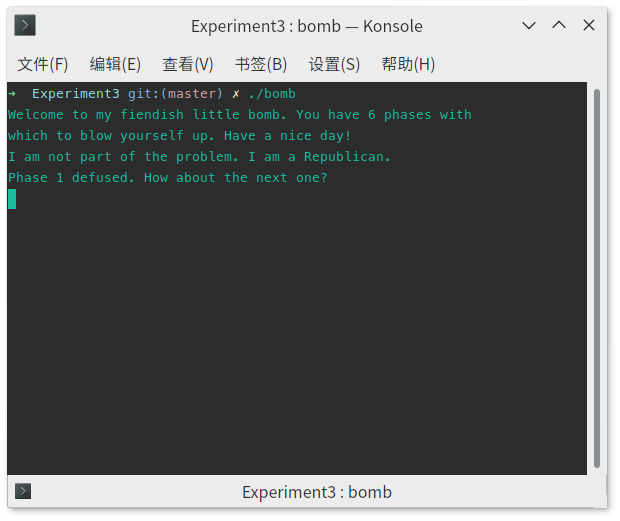
\includegraphics[width=\linewidth]{figures/Bomb-1}
\caption{阶段一}
\label{fig:bomb-1}
\end{minipage}
\begin{minipage}[r]{0.5\linewidth}
esi常作为参数使用,这里可以看到是比较字符串,推测0x402440是字符串地址,将其输出,发现确实是一串有意义的字符串,应该是答案一,测试成功。
\end{minipage}
\end{figure}


\subsection{阶段2的破解与分析}

\textbf{密码如下:}1 2 4 8 16 32

\textbf{破解过程:}

\begin{figure}[H]
    \begin{minipage}[l]{0.4\linewidth}
        \centering
        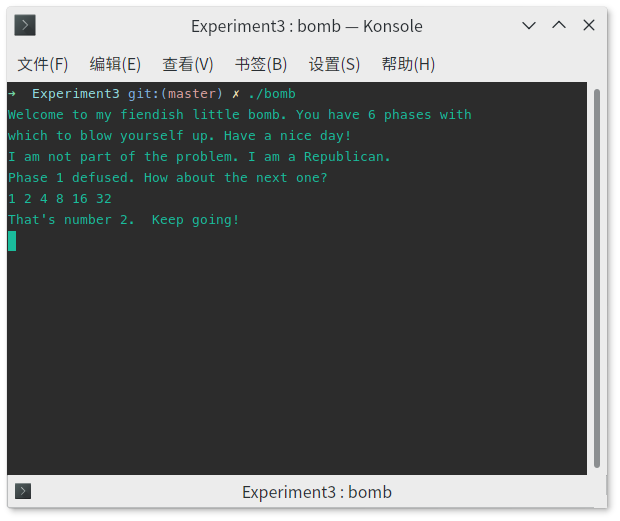
\includegraphics[width=\linewidth]{figures/Bomb-2}
        \caption{阶段二}
        \label{fig:bomb-2}
    \end{minipage}
    \begin{minipage}[r]{0.5\linewidth}
        看其汇编代码可知要我们输入的是6个数字,在读数完成之后可以发现,将rsp中的数据与1做了比较,不相等则爆炸,推测输入的地一个数字应该是1,之后则将eax赋值为ebx指向的值为1,在不读取完6个数字之前,每次eax做循环都会变成自己的2倍,然后与数组中的数据做比较,可得密码是1 2 4 8 16 32。
    \end{minipage}
\end{figure}

\subsection{阶段3的破解与分析}

\textbf{密码如下:}0 d 104

\textbf{破解过程:}

\begin{figure}[H]
\begin{minipage}[c]{0.4\linewidth}
\centering
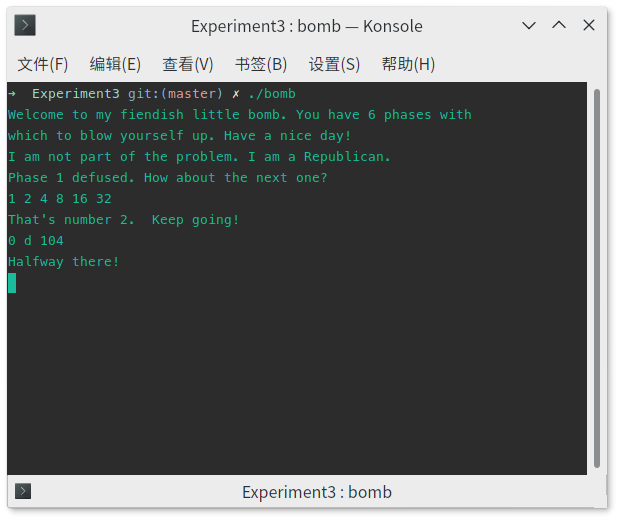
\includegraphics[width=\linewidth]{figures/Bomb-3}
\caption{阶段三}
\label{fig:bomb-3}
\end{minipage}
\end{figure}

\begin{lstlisting}
0000000000400f0d <phase_3>:
400f0d:	48 83 ec 28          	sub    $0x28,%rsp
400f11:	64 48 8b 04 25 28 00 	mov    %fs:0x28,%rax
400f18:	00 00 
400f1a:	48 89 44 24 18       	mov    %rax,0x18(%rsp)
400f1f:	31 c0                	xor    %eax,%eax
# sscanf 将值存入到 rsp+14 rsp+16 rsp+10里面去了
# 只需要看这这三个值即可
# sprintf(in,"%d %c %d",%rdx,%rcx,%r8)
400f21:	4c 8d 44 24 14       	lea    0x14(%rsp),%r8
400f26:	48 8d 4c 24 0f       	lea    0x0f(%rsp),%rcx
400f2b:	48 8d 54 24 10       	lea    0x10(%rsp),%rdx
# 0x40249e 是"%d %c %d" 这就是要输入的三个值
400f30:	be 9e 24 40 00       	mov    $0x40249e,%esi
400f35:	e8 76 fc ff ff       	callq  400bb0 <__isoc99_sscanf@plt>
# 成功输入三个值,否则爆炸 %eax=3
400f3a:	83 f8 02             	cmp    $0x2,%eax
400f3d:	7f 05                	jg     400f44 <phase_3+0x37>
400f3f:	e8 82 05 00 00       	callq  4014c6 <explode_bomb>
400f44:	83 7c 24 10 07       	cmpl   $0x7,0x10(%rsp)
# rsp+10>7就爆炸
400f49:	0f 87 f2 00 00 00    	ja     401041 <phase_3+0x134>
# 把第一个数存到eax
400f4f:	8b 44 24 10          	mov    0x10(%rsp),%eax
# 0x4024b0的值是0x400f5a 
# 跳转到0x400f5a + rax * 8 (rax < 7)
# Switch 通过输入的第一个值进行跳转 这里输入0
400f53:	ff 24 c5 b0 24 40 00 	jmpq   *0x4024b0(,%rax,8)
# 0 :
# 0x68 : %d 第二个数字 0x68 = 104
400f5a:	b8 64 00 00 00       	mov    $0x64,%eax
400f5f:	83 7c 24 14 68       	cmpl   $0x68,0x14(%rsp)
400f64:	0f 84 e1 00 00 00    	je     40104b <phase_3+0x13e>
400f6a:	e8 57 05 00 00       	callq  4014c6 <explode_bomb>
400f6f:	b8 64 00 00 00       	mov    $0x64,%eax
400f74:	e9 d2 00 00 00       	jmpq   40104b <phase_3+0x13e>
# -*- 其它选项 -*-
# 将中间字母和al做比较
# 输入 0 : %eax = %al = 0x64 = d 中间的字母是 d
# 答案 0 d 104
40104b:	3a 44 24 0f          	cmp    0xf(%rsp),%al
40104f:	74 05                	je     401056 <phase_3+0x149>
\end{lstlisting}

\subsection{阶段4的破解与分析}

\paragraph{密码如下:}

\paragraph{破解过程:}

\subsection{阶段5的破解与分析}

\paragraph{密码如下:}

\paragraph{破解过程:}

\subsection{阶段6的破解与分析}

\paragraph{密码如下:}

\paragraph{破解过程:}

\subsection{阶段7的破解与分析(隐藏部分)}

\paragraph{密码如下:}

\paragraph{破解过程:}
